\documentclass[12pt]{article}
\usepackage[margin=1in]{geometry}
\usepackage{timeline}
\usepackage{graphicx}
\usepackage{color}
\usepackage{float}
\usepackage{hyperref}
\usepackage{mathtools}

\usepackage[style=authoryear, backend=bibtex]{biblatex}
\addbibresource{final_bib.bib}
\nocite{*} 

\usepackage{listings}
\lstset{ %
language=Java,                % choose the language of the code
basicstyle=\footnotesize,       % the size of the fonts that are used for the code
numbers=left,                   % where to put the line-numbers
numberstyle=\footnotesize,      % the size of the fonts that are used for the line-numbers
stepnumber=1,                   % the step between two line-numbers. If it is 1 each line will be numbered
numbersep=5pt,                  % how far the line-numbers are from the code
backgroundcolor=\color{white},  % choose the background color. You must add \usepackage{color}
showspaces=false,               % show spaces adding particular underscores
showstringspaces=false,         % underline spaces within strings
showtabs=false,                 % show tabs within strings adding particular underscores
frame=single,           % adds a frame around the code
tabsize=2,          % sets default tabsize to 2 spaces
captionpos=b,           % sets the caption-position to bottom
breaklines=true,        % sets automatic line breaking
breakatwhitespace=false,    % sets if automatic breaks should only happen at whitespace
escapeinside={\%*}{*)}          % if you want to add a comment within your code
}

\author{Advisor/Client: Dave Hale \\ Team Members: Colton Kohnke}
\title{GPGN438 Senior Design: \\ Exploratory Seismic Data Analysis in the Field}
\date{April 28th, 2014}

\begin{document}
\maketitle
\newpage

\section{Executive Summary}

Seismic surveys take a significant amount of time and money to complete correctly. This project developed software for the Colorado School of Mines (CSM) to aid with viewing seismic survey data and geometry in the field. The software is also able to help catch errors in the field. It can serve as a teaching tool for the students of the Colorado School of Mines Geophysics Field Camp to help them better understand seismic surveys. \\

The software accomplishes this by reading the SEGD files from the Sercel recording truck along with the station locations from a GPS unit. This data is then plotted in map and section view in order to give snapshots of the seismic survey. The survey can then be explored in map view as stations and the shot records can be displayed based off of user input. This exploration comes in the form of dynamic display of shot records, stack of shot records and common channel sections.\\

Basic processing can then be completed in a dynamic and interactive way. The current included processes are gain, lowpass filtering, and time-power amplitude-gain. The program handles the display of the processed data with a user controlled slider for the processes. The plot of the selected data is updated in real-time as the user moves the slider. \\

The software is ready for use in the 2014 Geophysics field camp. The

\newpage
\tableofcontents
\listoffigures
\listoftables
\newpage

\section{Problem Statement}

This project seeks to develop software in Java that aids with the exploration of seismic data in the field. The survey exploration includes the interactive display of survey geometry and seismographs. This software will also be able to perform simple processing tasks in the field. The program will serve as a bridge from the seismic crew to the students of Field Camp and serve as a teaching tool for the student's understanding of the seismic survey.

\section{Introduction \& Background}

Geophysical data collection is an expensive operation that costs both time and money. In the field, it is in the data collector's best interest to make sure that the data collected is high quality. Poor data collection can waste time in the field and hinder processing when back in the office. \\

ProMAX is the current system used in the field to view the seismic data coming in from the recording station. This system, while good for extensive processing, is not robust enough to quickly display survey data and interactively display the survey geometry. The CSM Field Camp is unique in that they surveys are not conventional, that is, the surveyors are trying parameters or setups that aren't typical of a corporate survey. This makes the data look unconventional and causes problems during standard processing. \\

There can also be a lack of understanding between the students and the seismic survey with regards to how the data is collected in the field. This software will seek to help the students at Field Camp better understand the seismic survey while they are in the field. The software can also be used as a teaching tool to the students in Field Camp to help them better understand the aspects of a seismic surveys.

\section{Deliverables to Client}

The deliverables of this project include two main items. The first is a program written in Java that accomplishes the design objectives outlined in the next section. The second deliverable will be a documentation of the code in the standard Java practices and a compilation of the documentation using the Javadoc tools provided by Sun Microsystems. 

\section{Design Objectives}
\subsection{Interactive Display of Survey Geometry}

The first objective is to be able to import station (flag) locations. This needs to be accomplished from a variety of GPS sources including CSV, Garmin GPX and tab-delimited text files. The GPS coordinates need to then be converted to UTM for display. Once these stations have been imported and converted, they need to have the option of being exported so the conversion does not need to be applied again. The columns for export are listed in Table \ref{TAB:GPS}. Once the conversion is applied, the next step is to plot the locations in map view.

\begin{table}[H]
\caption{GPS Export Spreadsheet Fields}
\centering
\begin{tabular}{ c | c | c | c}
  \hline                  
  StationID & UTM Easting & UTM Northing & Elevation \\
  \hline
\end{tabular}
\label{TAB:GPS}
\end{table}

The second objective is to be able to compute source and receiver locations. This is done for each valid shot FFID (Field File ID) by using the Sercel SEGD files to determine the source station number, live recording channels and receiver station numbers. The station locations are then used to find the location of the source and the elevation is read from a USGS Digital Elevation Map. Some FFIDs correspond to bad shots and will need to be ignored dynamically by the program routines. \\

Once the data has been extracted from the SEGD files, the program needs to be able to plot source and receiver locations in map view. The program also needs to be able to plot elevation profiles along the source and receiver lines. Finally, there needs to be a slider to select and show points corresponding to each FFID that will provide a graphical history of the seismic survey and help to catch mistakes. 

\subsection{Interactive Display of Seismograms}

The first step to displaying the seismograms is to convert the SEGD files (bytes) to an array of an array of floats (2D float array). Once this is accomplished, the seismograms need to be interactively displayed by using the mouse in map view. Another method of display will be to display all seismograms within a circle that the user draws in map view. \\

\subsection{Interactive Gain, Amplitude Balancing and Lowpass Controls}

All of the displays are unless the data can be seen. Therefore, interactive controls for gain, amplitude balancing and lowpass filtering (Butterworth) need to be implemented and the results plotted. This will be done by using sliders embedded in the graphical user interface. As the user moves the slider, the response plot updates in real time.

\subsection{Other Requirements}

Speed is a top priority when working in the field. Decisions are typically made quickly in order to move the survey along at a reasonable rate. If this software is fast enough, it can be used as a supplement to those decisions. The field camp data is small enough that speed should not be an issue. \\

The user-interface must be easy to use. The layout of the controls must be logical and follow a sequential order. These different features must be documented in the end-user documentation and be consistent in their implementation. If there are errors thrown in the process of importing and plotting the data, the user needs to be made aware of the steps they are missing.

\section{Decision-making \& Assessment of Alternative Approaches}

The decisions during the main software development section of this project deal with efficiency. It is possible that choices in the field need to be made quickly and as a result, the software needs to be able to perform operations efficiently to keep pace. If the software is called to display a seismic shot, it needs to be able to find the data and display it in the least amount of operations. Similarly, if an operation is applied to a set of data, it should be applied in the least amount of compute time. \\

The software is not currently optimized for speed because that would slow down development. However, specific places in the software have been marked for efficiency improvements during the testing phase. One area that has been marked for optimization is the storage of the data from the SEGD files. Currently, shots are stored as an ArrayList which is traversed linearly. This causes an O($n^2$) search time where $n$ is the length of the array. A much faster implementation would be a Binary Search Tree which has O($n$) traversal time. Another option is implementing a hash table, which returns a value in near constant time, O($1$). \\

The decisions during the later stages of the project revolve around end user usability. These choices will include aesthetic placement of tools in the software to create a logical progression of tasks for the end user. The decisions in this section will also revolve around how to lay out the documentation for the end user. These decisions will be made during the final stages of the project and will involve talking with the client to find a pleasing layout. \\

\section{Design Solution}

The tool that is being used in this design project is simulation. Each method that is written is tested by calling a main method that tests against the 2013 Field Camp data. These simulations provide the developer with real data to test the software against and provides speed/efficiency benchmarks to improve upon. \\

In addition, before a feature is integrated into the larger code, it is tested against itself for errors and correct implementation. This speeds up the development process because it limits the area where bugs can occur at any given time. When the bugs occur, they are fixed in the responsible code and retested for consistency.

\section{Implementation Plan}
\subsection{Safety}

The main safety concern of this project is the ergonomics of the developer. This project does not require field work or manual labor in the traditional sense. However, it does require a significant amount of time to be spent coding at a computer which may cause irritation of the wrist or forearm. The developer will mitigate the risk of encountering this problem by taking breaks, stretching and using correct posture while at the workstation.

\subsection{Timeline}

\begin{figure}[H]

\begin{timeline}{2013}{2015}{200}{300}
  \categorylabel{Senior Design Timeline}{60}
  
  \MonthAndYearEvent{9}{2013}{Project start}
  \MonthAndYearEvent{10}{2013}{Java base using Mines JTK Demo files.}
  \MonthAndYearEvent{11}{2013}{Sercel SEGD reading and plotting Jython code converted to Java.}
  \MonthAndYearEvent{11}{2013}{Demo with interactive plots created}
  \MonthAndYearEvent{1}{2014}{Core features implemented}
  \MonthAndYearEvent{1}{2014}{Alpha testing starts}
  \MonthAndYearEvent{1}{2014}{Code optimization begins}
  \MonthAndYearEvent{3}{2014}{Beta testing begins}
  \MonthAndYearEvent{3}{2014}{Documentation writing begins}
  \MonthAndYearEvent{5}{2014}{Final product ready for use at CSM Field Camp 2014}
  
\end{timeline}
\caption{Senior Design Project Timeline}
\end{figure}

\subsection{Budget 1: Actual}

No budget is required for the actual project as the project does not require any traveling or other expenditures outside the realm of a standard class at CSM.

\subsection{Budget 2: Professional}

Ideally to get a working product to the client, the following budget in Table \ref{TAB:BUG} would be used in a professional setting. 

\begin{table}[H]
\caption{The Professional Budget}
\begin{tabular}{ l | l | l || l | l}
  \hline                        
  Item & Base Cost & Quantity & Total & Notes \\ \hline
  Developers & \$20.00/hr & 360 & \$7,200 & 2 Devs for 4 work weeks.\\
  Continued Support & \$15.00/hr & 260 & \$3,900 & 1 Dev at 5 hours/week for 1 year.\\ \hline
  Base Total & & & \$11,100 & \\
  Overshoot & & & \$1,110 & 10\% addition\\ \hline
  Total & & & \$12,210 & \\
  \hline  
\end{tabular} 
\label{TAB:BUG}
\end{table}

In reality, a project of this magnitude would likely cost much more than anticipated above. The main cost is dependent on the size of the team developing the program, their skill level, and what features are being implemented. These extra variables make discerning an actual budget more complicated. On a related note, the project could potentially be funded by selling the program to clients. To market this program, more hurdles would have to be overcome and an expanded budget would be created.

\section{Program Design}

The program is divided into several levels of command to aid further development. The highest level, PlotTest, initiates the program by constructing the three plots. The three plots act as secondary controllers to the program. Finally, there are multiple helper classes that aid the three plots in calculating and obtaining data. \\

In a hierarchical sense, the PlotTest class can be compared to the King of a large kingdom and the three plot classes are the King's Counsel. The Counsel talks freely with each other and give each other objectives to accomplish. Each Counsel member reports directly to the King, who will then order the Counsel to complete further action. The program contains a variety of helper classes that assist the King and Counsel in gathering the data that they need to import or plot. These helper classes exist outside the realm of the the plots and are able to gather and import data autonomously to the controlling classes.

\subsection{Main Controller - PlotTest Class}

The Main Controller of the program is the PlotTest Class. Inside the PlotTest class, there exist secondary classes for the different plotting frames. The PlotTest class is responsible for storing data that is imported, creating menu items, and for handling different modes for the plots. The PlotTest class is also responsible for taking information passed to it by its internal classes (BasePlot, ResponsePlot and ElevPlot) and then telling them to do the next routine. \\

\subsubsection{Menu Items}

The first Menu is the "File" Menu. Under this header, there are two options. The first option is "Save as PNG"  which will bring up a file browser (Figure \ref{FIG:PNG}) that will save the current plot to a PNG image file. The plot that is saved will be the plot from the window that the menu item is selected from.

\begin{figure}[H]
\centering
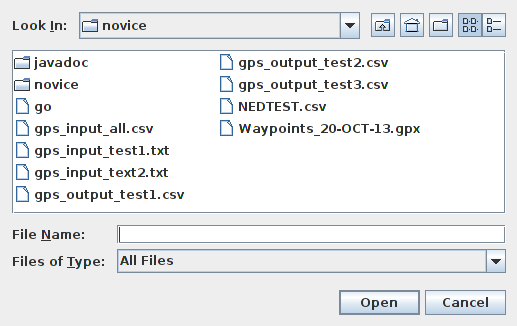
\includegraphics[width=0.75\textwidth]{./figs/fig0.png}
\caption{JFileChooser for importing data.}
\label{FIG:PNG}
\end{figure}

The second option under the "File" menu is "Exit," which will close the program and end clear all memory. \\

The second Menu is the "Mode" menu. This menu allows for switching between the various modes that are available. At the time of this writing, the modes that exist are "Zoom Mode," "Roam Mode," "Circle Mode" and "Channel Mode." Each Mode has a different function for the various plots, and their role will be discussed in those sections. The Modes also have icons on the right side of the base map. \\

The "Tools" Menu contains methods to import and manipulate data. The "Get HandHeld GPS" option will import GPS points from a Tab Separated Value (TSV), Comma Separated Value (CSV) or Garmin GPX file. The file type is automatically detected based on the data file extension. This routine assumes that the TSV and CSV data is of a format similar to Table \ref{TAB:GPS2}. Currently, any elevation values are ignored in favor of Nation Elevation Database (NED) files. Also, the data must be in decimal latitude and longitude and will be converted to UTM Easting and Northing upon import. Importing GPS data will update the Base Map plot with the points.\\

\begin{table}[H]
\caption{GPS Import Spreadsheet}
\centering
\begin{tabular}{ c | c | c}
  \hline                  
  Station ID & Latitude (decimal) & Longitude (decimal) \\
  \hline
\end{tabular}
\label{TAB:GPS2}
\end{table}

The next item is "Import NED Files" and it adds the NED GridFloat files to the PlotTest's list of NED files to search through. In Pagosa, the seismic survey was located on the edge of two NED files, so the program was written to be able to handle multiple NED files. This method requires the GridFloat file (extension ".ftl") to be in the same directory as the Header file (extension ".hdr"). \\

"Read Elevations from NED" will take the current imported GPS points and the imported NED Files and update the GPS point elevation fields. This happens based on the GPS point's latitude and longitude. The Elevation plot is then updated with the result. \\

"Export GPS to CSV" will export the GPS data to a CSV file. The format of the export is defined in Table \ref{TAB:GPS}. Exporting the data will not erase the data stored in memory. \\

"Import Segd Directory" will open up a file browser and when the user selects a directory, all of the Segd files (extension ".segd") of Sercel's format will be read and imported into memory. "Import Segd File(s)" does the same thing, but the user must specify a specific Segd file to import. \\

The "Test" Menu item contains methods that the developer was testing before integrating into a different Menu. The current test items are "Display Range," "Clear Data" and "Plot Controls." "Display Range" is obsolete and is marked for deletion. "Clear Data" is for making testing easier and it clears the storage for Segd data, GPS data and NED files. Finally, "Plot Controls" displays sliders that are used for controlling the gain, lowpass filtering and the amplitude balancing. More information on the "Plot Controls" item is discussed in the ResponsePlot section below.

\subsection{Secondary Controller - BasePlot Class}

The main purpose of the BasePlot class is to display the survey in map view. The other purpose of this plot if to allow for exploration of the seismic survey in a dynamic environment. 

\begin{figure}[H]
\centering
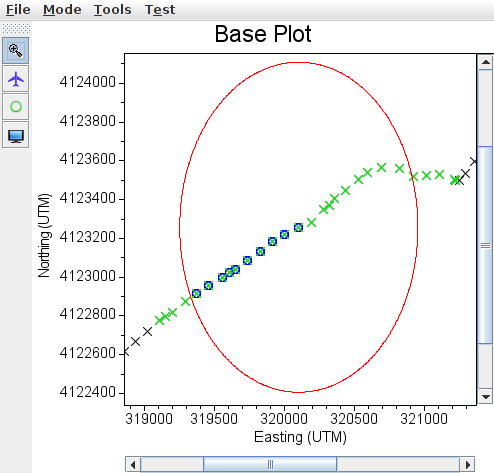
\includegraphics[width=0.75\textwidth]{./figs/fig1.png}
\caption{The base map after GPS and SEGD data has been imported during Roam Mode with summation turned on. This plot shows selected shots (the blue circles inside the red circle), the active receiver locations (green crosses) and the station locations (black crosses).}
\label{FIG:BP}
\end{figure}

In Figure \ref{FIG:BP} we see the map view of the GPS in Roam Mode and a distance of summation defined. The legend for this plot is independent of mode and defined as follows. The black cross icons define where the GPS points are located. The blue circles define which shots are currently selected. The green crosses define the receivers that are currently active. The red circle defines the range of shots that are being plotted by the response plot.

\subsubsection{Zoom Mode}

In Zoom Mode, the base map may be zoomed in and explored using the scroll bars. This allows for a specific part of the seismic survey to be highlighted. To zoom, click and drag a box of interest and then let go of the mouse to zoom. To zoom out to the default view mode, right click the mouse. 

\subsubsection{Roam Mode}

When Roam Mode is selected, the user can click as drag their mouse along the seismic line in order to display the shot records. The shot record that is displayed in the Response Plot is dependent on the user's current mouse location. The program will determine the closest GPS station to the mouse and then determine the nearest shot to that GPS location for display. The response plot updates in real time as the user moves their mouse. At any time, the user may change the Summation Range Slider to display more (or less) combined shot records. The summation is based from the closest GPS point, meaning in locations with no data, no shot records will be combined.

\subsubsection{Circle Mode}

Circle Mode behaves much like Roam Mode, but instead of click and dragging the mouse to display the nearest shot, the user clicks and drags to define a circular range. As the user moves their mouse to define a range, the base map and the response plots will update with what shots are within that range, what receivers are active and the brute stack of the selected shots. The first point the user defines is the center of the circle and from there, they define the radius. In most cases, the circle will actually be elliptical due to the scale of the axes.

\subsubsection{Channel Mode}

The user can use Channel Mode to create a common channel section. In this mode, a slider appears that can be used to update the response plot in real time. The slider is created each time this mode is activated with the maximum channel number of the data that has been imported. If the channel does not exist at a certain receiver location, the response plot will have a vertical black line at the receiver location.

\subsection{Secondary Controller - ResponsePlot Class}

The ResponsePlot Class is responsible for the plotting of the seismic data. Depending on the mode, different types of plots are created.  In the case of Roam Mode and Circle Mode, a brute stack of selected shots is displayed. In the case of Channel Mode, a common channel section is created. Figure \ref{FIG:RP} shows a standard display in Roam Mode with no summation or in Circle Mode with only one selected shot.

\begin{figure}[H]
\centering
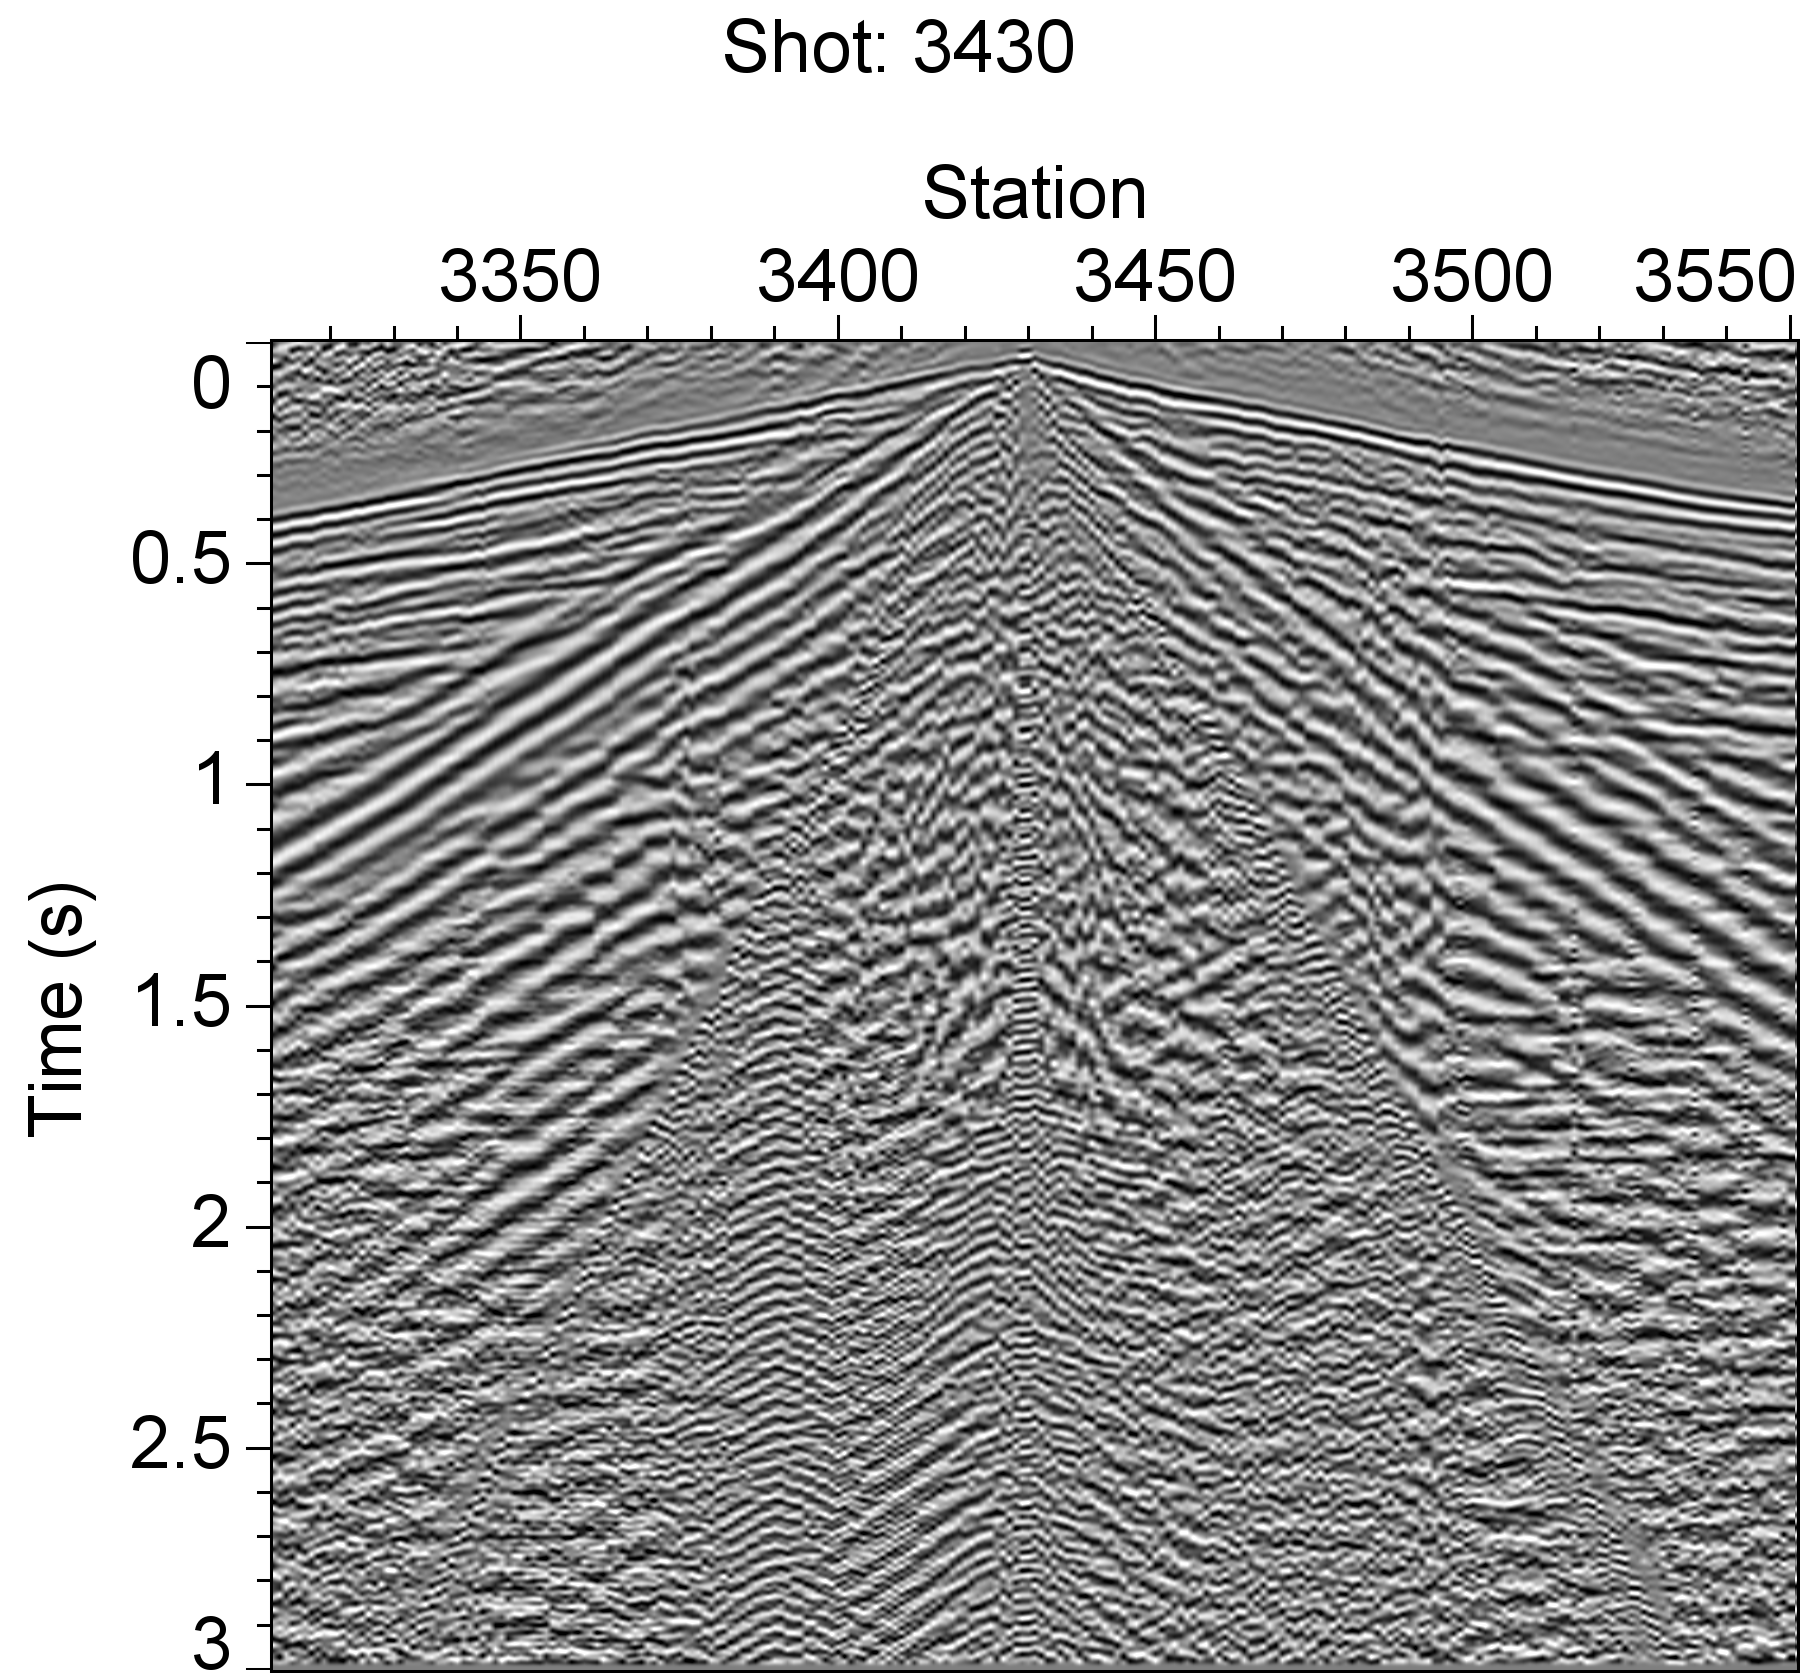
\includegraphics[width=0.75\textwidth]{./figs/fig4.png}
\caption{The Response Plot during Roam Mode with no summation. This shows a single shot record.}
\label{FIG:RP}
\end{figure}

\subsubsection{Zoom Mode}

In Zoom Mode, the base map may be zoomed in and explored using the scroll bars. This allows for a specific part of the seismic shot to be highlighted. To zoom, click and drag a box of interest and then let go of the mouse to zoom. To zoom out to the default view mode, right click the mouse. 

\subsubsection{Roam Mode}

The response plot in Roam Mode will dynamically update based on the user's actions on the base plot. If the user clicks on the base map, the response plot will show the nearest shot record. If the user clicks and drags, the response plot will update in real time with the nearest shot. If the user slides the summation slider, the response plot will update with a stack of the shots within range.

\begin{figure}[H]
\centering
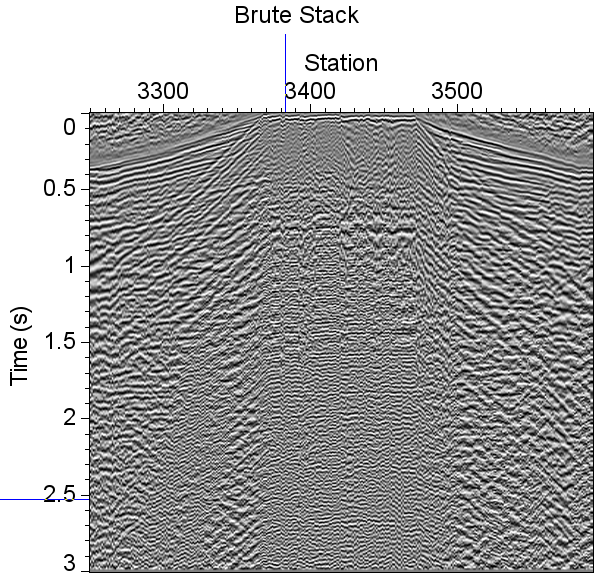
\includegraphics[width=0.75\textwidth]{./figs/fig3.png}
\caption{The Response Plot during Roam Mode showing an example stacked section.}
\label{FIG:RPR}
\end{figure}

\subsubsection{Circle Mode}

The response plot behaves the same way in Circle Mode as in Roam Mode. As the user expands the circle to encompass more shots on the base plot, a brute stack is created with the selected shot records. 

\subsubsection{Channel Mode}

Channel Mode has to behave the same way as the other two Modes. However, in Channel Mode, the response plot has to update itself based on a slider that the user controls. A sample image of what to expect with a Common Channel Section would look like in the response plot is seen in Figure \ref{FIG:RPC}.

\begin{figure}[H]
\centering
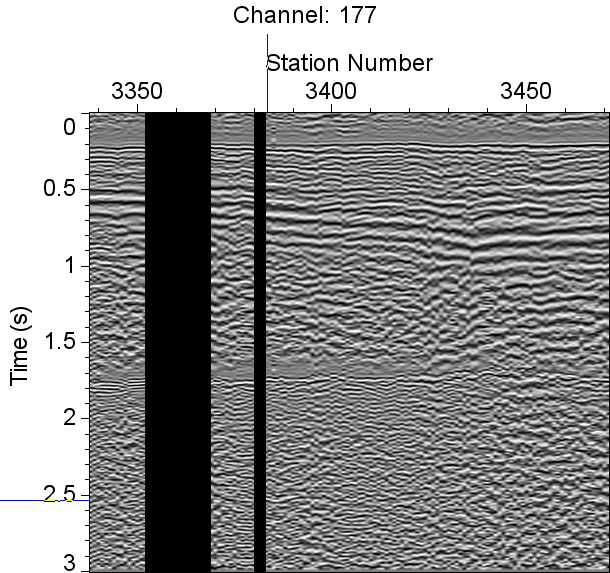
\includegraphics[width=0.75\textwidth]{./figs/fig5.png}
\caption{The Response Plot displaying a common channel section in Channel Mode.}
\label{FIG:RPC}
\end{figure}

\subsection{Secondary Controller - ElevPlot Class}

The elevation plot is controlled by the ElevPlot Class. When the GPS is first imported, the elevation plot updates. Then when the elevations are updated from the NED files, the elevation plot updates again. Figure \ref{FIG:EP} shows what the elevation plot looks like after the GPS and the NED files have been imported and the NED files read.

\begin{figure}[H]
\centering
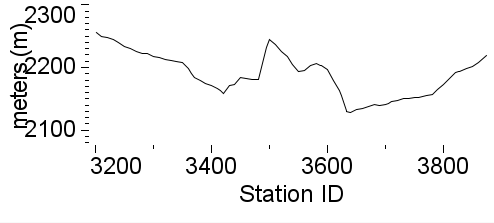
\includegraphics[width=0.75\textwidth]{figs/fig2.png}
\caption{Sample of the Elevation Plot profile after the NED files have been imported and read.}
\label{FIG:EP}
\end{figure}

\subsection{Helper Modules - MPoint \& Waypoints Classes}

The MPoint and the Waypoints classes deal with GPS points. An MPoint is essentially a map point with private fields for location in UTM and Lat/Lon coordinates. The MPoint class also includes methods for determining the distance between two MPoints. This is useful when trying to determine if an MPoint lies within a range of another MPoint (such as in Circle Mode). \\

Waypoints include methods for dealing with collections of MPoint objects. The methods in Waypoints includes tools for importing and exporting MPoint collections from and to files respectfully. Waypoints also has methods for determining the minimum and maximum station number. Waypoints also has a way of converting the lat/lon of a collection of MPoints into UTM easting and northing. 

\subsection{Helper Modules - NedFile, NedFileHeader \& NedFileReader Classes}

The NedFile, NedFileHeader and NedFileReader Classes are are used for importing and reading NED files. The NedFile is composed of information about the north and west limits of the GridFloat file (extension ".ftl"). The NedFileHeader is where the information about the actual NedFile data is read and stored; that is, information such as the GridFloat file's cell size, lower left corner, and erroneous values. This all comes from the header file of the GridFloat file (extension ".hdr"). The NedFileReader class contains methods for reading the GridFloat file and extracting an elevation. This class does not interpolate between points and instead assumes elevation is constant for each cell. 

\subsection{Helper Modules - Segdata \& Segd Classes}

The final helper helper modules have tools for reading and storing data that is pulled from Segd files (extension ".segd"). The Segdata class is used to store the information about a particular shot. The important information includes the shot number (which is the same the GPS point), the line number, the beginning receiver station, the ending receiver station and the 2D array of the shot record. The Segd class includes tools for manipulating a list of Segdata objects including tools for importing the Segd files. Segd also includes tools for gaining, amplitude balancing and lowpass filtering the data.  

\section{Discussion and Conclusions}

This project developed robust software in Java that aids with the exploration of seismic data in the field. The program that was developed includes the interactive display of seismic survey geometry and shot records. This software is also able to perform simple processing tasks such as gain, amplitude correction, and lowpass filtering in the field. The program can also calculate and display brute stacks over a range of shots.  \\ 

While the program is far from an industry level program, it is a great start to a helpful field program. The documentation will aid future development and help the field camp students 

\section{Recommendations for Future Work}

The recommendations for future work fall into the categories of code cleanup and feature addition. The code cleanup will help with efficiency, speed and further development. Feature additions will help make the more useful in the field. 

\subsection{Code Reorganization}

\begin{itemize}
\item More separation of PlotTest and its internal classes. Currently, the PlotTest class is composed of multiple inner. This can cause confusion when developing because it may not be clear to the programmer what parts of the code control what parts of the plot. It's my suggestion to separate the Plot classes from inside the PlotTest class. From here, the PlotTest class can function more as Main Controller with absolute control over everything and less of a Controller with shared power with its inner classes.

\item Optimization of search features. Currently the search algorithms used to find specific shots and map points is linear through a list. In order to maximize efficiency, a Binary Search Tree (BST) or Hash Map should be used.

\item Currently, the seismic survey's sampling rate is a constant 0.002 s/sample. This can easily change depending on the survey. There needs to be a way to change this value in the program so the plots and processing can be useful in other survey parameters.
\end{itemize}

\subsection{Feature Addition}

\begin{itemize}

\item Reading and processing of observation reports. There is a whole set of data that has not been utilized for this program. The inclusion of such data could tell the user which channels are active and how much offset the shots have from the GPS station.

\item Expand the segd data import tool to include non-Sercel seismic. This would require diving into different acquisition company's method of storing seismic data and programming logic to detect the type. A possible resource for this would be the Seismic Unix source code.

\item The ability to view ResponsePlot without GPS with a slider for shot number. In some cases, the GPS data might be acquired after the seismic data starts shooting. In these cases it would be helpful to still be able to view the seismic data by using a slider to display certain shot numbers. The current system is too dependent on GPS data for this type of robust viewing.

\item Extra tools for processing (kill ground roll, NMO correction, etc.). The python code provided by the client has several programs that are able to accomplish more processing that what is currently implemented. The reason these were not implemented in the current working version was due to time constraints.

\item GPS needs more robust import/export system (needs "specific" format). The current regime only allows for very specific GPS formats to be imported. In order to be more robust, the user should be able to define how the GPS data they want to import is structured. The same should be true of exporting GPS data.

\item A UTM to Lat/Lon conversion. Currently the only supported mode for displaying GPS data is when it is in UTM coordinates. However, the only way to read the NED files is if the GPS data has lat/Lon components. This could potentially cause a major issue if the GPS data is not read in as Lat/Lon data. 

\item A "save state" button. It would be helpful if the when the user closed down the program they could easily relaunch the program in the state they left it in. This may not be easily feasible because of the size of seismic surveys and the data storage requirements. 

\item The Elevation Plot should be more integrated into the activities on the base map. The elevation plot should have similar features as the base map. Active shots should be coded with blue circles, active receivers with green crosses and the range of shots with a red line.
\end{itemize}

\newpage
\section{References}

\printbibliography

\newpage
\section{Team Resume}

*to be added*

%% LaTeX file for resume 
% This file uses the resume document class (res.cls)

\documentclass[margin]{res}
%\usepackage{helvetica} % uses helvetica postscript font (download helvetica.sty)
%\usepackage{newcent}   % uses new century schoolbook postscript font  
\topmargin=-0.6in  % start text higher on the page
\setlength{\textheight}{11in} % increase text height to fit resume on 1 page
\usepackage{color}

\begin{document}  
\name{COLTON KOHNKE}
\address{1221 Illinois Street Apt. 2E \\ Golden, CO 80401 \\ (360) 813-2795 \\ ckohnke@mines.edu }

\begin{resume}                        

\section{EDUCATION} \textbf{Colorado School of Mines, Golden, CO} \hfill B.S. May 2014 \\
                Geophysics \& Geophysical Engineering \hfill CUM GPA 3.46 \\
                \textcolor{white}{...} \hfill Major GPA 3.61 \\
                \textbf{Professional Organizations}
                \begin{itemize}
                 \item Society of Exploration Geophysicists Student Member (SEG)
                 \item European Association of Geoscientists and Engineers (EAGE)
                \end{itemize}

\section{WORK \\ EXPERIENCE}
		  %\begin{tabular}{p{3in} r} 
			\textbf{Chevron of North America, Bakersfield, CA} \hfill Summer 2013 \\
			Upstream Technical Computer G{\&}G Support Intern
		  		\begin{itemize}
		  		\item Designed, developed, documented and deployed a new error reporting system to ensure well data integrity between 						multiple databases.
		  		\item Assessed opportunity of a new database/software system for seismic metadata to increase efficiency and safety while decreasing cost.
		  		\item Worked with Data Analyst and Asset Development teams to standardize well status symbols for use within the San Jaoquin Valley.
		  		\end{itemize}
		  		
			\textbf{Ventyx, Greenwood Village, CO} \hfill Summer 2012 - June 2013 \\
			MineScape Engineer Intern
                  %\end{tabular}	
                   \begin{itemize} % \item[] prevents a bullet from appearing
                    \item Wrote, debugged, tested and integrated code into MineScape software.
                    \item Tested the new MineScape 5.4 release.
                    \item Traveled and assisted clients with overburden stratigraphic modeling and \\geophysical interpretation on an 							open-pit coal mine.
                    \item Wrote and updated documentation for consumer utilization.
				   \end{itemize} 

\section{ENGINEERING \\ \& TECHNICAL \\ SKILLS} 
		\begin{itemize}
		\item MineScape, MineScape Programming Language, Geolog, OpenWorks, Petrel.
		\item JAVA/C++, MatLab, Python, R, LaTeX, and Mathematica.
		\item Geological Lab Experience, Geophysical Field Methods, Geophysical Survey \\ Design, GPS, Field and Office Safety, Well-Log Analysis.
		\item AutoCAD, SolidWorks; Microsoft Excel, Word, Powerpoint, Publisher.
		\item Linux/UNIX, Windows, and Mac OS.
		%\item Finite Element Analysis, Systems, Computer Aided Data Acquisition, Graphical and Written Design Proposals, Oral Presentation, Technical Writing, Formal Proposal Writing, Budgeting, and Scheduling.
		\end{itemize}
		
\section{PROJECT \\ EXPERIENCE}
		  %\begin{itemize}
			 %\item
            \textbf{Senior Design: Exploratory Analysis of Field Seismic Data} - Senior capstone project written in JAVA to quickly and accurately analyze seismic data in a field setting. Features include an interactive display of survey geometry, seismograms and simple processing tools. Expanding features to include field data from other methods (gravity, magnetics, DC/SP, GPR, and EM) as time permits.
			 
			\textbf{Geophysics Field Camp 2013} - Project to characterize the geothermal potential of Pagosa Springs, CO. Involved two weeks in the field gathering Gravity, Magnetics, EM, GPR, DC/SP, and Seismic data. This was followed by two weeks of data processing and technical report writing. Conclusions were published by the Colorado School of Mines Department of Geophysics.
			 
		   %\textbf{EPICS II: Geophysics Design} - Projects involving use of data analysis tools, such as R and JAVA, to interpret 					various data sets to solve a problem. Projects included analysis of sunspot data, correlation of local snowfall data, 					well-log analysis and finding \\ major driving forces for change in Lake Powell's water depth.
		   
		   %\textbf{EPICS I: Playground for the Disabled in South Africa} - Project \\involving research, conceptual design, graphical 				representation, subsystem analysis, materials list and budget of a playground for disabled children. Finalist in the 				EPICS 			competition.
		  %\end{itemize}

\section{OTHER \\ EXPERIENCE}
		  \begin{itemize}
		    \item Advanced Engineering Math Grader - Fall 2013.
		    \item Expected JAVA course Teaching Assistant - Spring 2014.
			\item High Grade Literary Journal Poetry Editor.			
			%\item Colorado School of Mines Varsity Swim Team.
			%\item Co-Founder and Officer of Mines Urban Gaming Club.
			\item Colorado School of Mines Peer Mentor.
			%\item Employment with the YMCA \& CSM Student Recreation Center.
		  \end{itemize}

\section{HONORS} 
	\begin{itemize}
	 \item Newmont Mining Scholar.
	 \item Naval Dolphin Scholarship Foundation Recipient.
	\end{itemize}
	 
%\section{{EXTRA-CURRICULAR \\ ACTIVITIES}} 
%	\begin{itemize}
%	 \item 
%	\end{itemize}
	 
\end{resume} 
\end{document}











\newpage
\section{Appendices}

*to be added*

\end{document}